\documentclass[a4paper, fleqn]{article}
\usepackage[utf8]{inputenc}
\usepackage{amsmath}
\usepackage{amssymb}
\usepackage{caption}
\usepackage{mathtools}
\usepackage{amsfonts}
\usepackage{lastpage}
\usepackage{tikz}
\usepackage{float}
\usepackage{textcomp}
\usetikzlibrary{patterns}
\usepackage{pdfpages}
\usepackage{gauss}
\usepackage{fancyvrb}
\usepackage[table]{colortbl}
\usepackage{fancyhdr}
\usepackage{graphicx}
\usepackage{pdfpages}
\usepackage[margin=2.5 cm]{geometry}

\setlength\parindent{0pt}
\setlength\mathindent{75pt}

\definecolor{listinggray}{gray}{0.9}
\usepackage{listings}
\lstset{
	language=,
	literate=
		{æ}{{\ae}}1
		{ø}{{\o}}1
		{å}{{\aa}}1
		{Æ}{{\AE}}1
		{Ø}{{\O}}1
		{Å}{{\AA}}1,
	backgroundcolor=\color{listinggray},
	tabsize=3,
	rulecolor=,
	basicstyle=\scriptsize,
	upquote=true,
	aboveskip={0.2\baselineskip},
	columns=fixed,
	showstringspaces=false,
	extendedchars=true,
	breaklines=true,
	prebreak =\raisebox{0ex}[0ex][0ex]{\ensuremath{\hookleftarrow}},
	frame=single,
	showtabs=false,
	showspaces=false,
	showlines=true,
	showstringspaces=false,
	identifierstyle=\ttfamily,
	keywordstyle=\color[rgb]{0,0,1},
	commentstyle=\color[rgb]{0.133,0.545,0.133},
	stringstyle=\color[rgb]{0.627,0.126,0.941},
  moredelim=**[is][\color{blue}]{@}{@},
}

\lstdefinestyle{base}{
  emptylines=1,
  breaklines=true,
  basicstyle=\ttfamily\color{black},
}

\pagestyle{fancy}
\def\checkmark{\tikz\fill[scale=0.4](0,.35) -- (.25,0) -- (1,.7) -- (.25,.15) -- cycle;}
\newcommand*\circled[1]{\tikz[baseline=(char.base)]{
            \node[shape=circle,draw,inner sep=2pt] (char) {#1};}}
\newcommand*\squared[1]{%
  \tikz[baseline=(R.base)]\node[draw,rectangle,inner sep=0.5pt](R) {#1};\!}
\newcommand{\comment}[1]{%
  \text{\phantom{(#1)}} \tag{#1}}
\newcommand\vgap{\noalign{\vskip 0.1cm}}
\def\el{[\![}
\def\er{]\!]}
\def\dpip{|\!|}
\def\MeanN{\frac{1}{N}\sum^N_{n=1}}
\cfoot{Page \thepage\ of \pageref{LastPage}}
\DeclareGraphicsExtensions{.pdf,.png,.jpg}
\author{Nikolaj Dybdahl Rathcke (Student ID: 74763954)}
\title{Optimization - MATH412 \\ Assignment 3}
\lhead{Optimization - MATH412}
\rhead{Assignment 3}

\begin{document}
\maketitle
\newpage

\section*{Question 2}
\subsection*{(a)}
\begin{align*}
  min_{x,y}\frac{1}{2}(x^2+(y-1)^2) \\
  c(x,y)=y-ax^2=0
\end{align*}
Only two of the KKT conditions apply to this problem as we have no inequalities. These are primal feasibility:
\begin{align*}
  y-ax^2=0
\end{align*}
and the stationarity condition:
\begin{align*}
  \begin{bmatrix}
    \frac{\partial f}{\partial x} \\
    \frac{\partial f}{\partial y}
  \end{bmatrix}
  -\lambda
  \begin{bmatrix}
    \frac{\partial c}{\partial x} \\
    \frac{\partial c}{\partial y}
  \end{bmatrix}
  &=
  \begin{bmatrix}
    x \\
    y-1
  \end{bmatrix}
  -\lambda
  \begin{bmatrix}
    -2ax \\
    1
  \end{bmatrix}
  =
  0
\end{align*}
This gives us the $3$ equations:
\begin{align}\label{eq1}
  y-ax^2        &= 0 \\
  x+2ax\lambda  &= 0 \\
  (y-1)-\lambda &= 0
\end{align}
The Langrangian $L$ is given by:
\begin{align*}
  L&=f-\lambda c \\
   &=\frac{1}{2}\left(x^2+(y-1)^2\right)-\lambda \left(y-ax^2\right)
\end{align*}
It has the partial derivatives:
\begin{align*}
  \frac{\partial L}{\partial x} &= x+2ax\lambda \\
  \frac{\partial L}{\partial y} &= y-1-\lambda
\end{align*}
If the two equations above equal $0$ for some point $(x,y)$, it means $(x,y)$ is a
stationary point of $L$. These are the same as Equation (2) and (3), so any point that
satisfies all three equations must naturally also satisfy the last two and therefore must
be a stationary point of $L$.

\subsection*{(b)}
Solving for $x,y$ and $\lambda$ in the three equations from the above question gives the solutions:
\begin{align*}
  x &= 0, y= 0, \lambda = -1 \\
  x &=\frac{\sqrt{a-\frac{1}{2}}}{a}, y=1-\frac{1}{2a}, \lambda= -\frac{1}{2a} \mbox{ where }
  a\neq 0 \\
  x &=-\frac{\sqrt{a-\frac{1}{2}}}{a}, y=1-\frac{1}{2a}, \lambda= -\frac{1}{2a} \mbox{ where }
  a\neq 0
\end{align*}
When $a<1/2$, the square root term for $x$ in the Equation (2) and (3) becomes imaginary
giving us only one real solution. When $a=1/2$, all three solutions are the same. If
$a>1/2$, the square root is real and therefore we have three real solutions.

\subsection*{(c)}
The sketch of the level curves and the constraint for $a=\{1/3,1/2,1\}$ is seen in Figure
\ref{fig1}:
\begin{figure}[H]
  \centering
  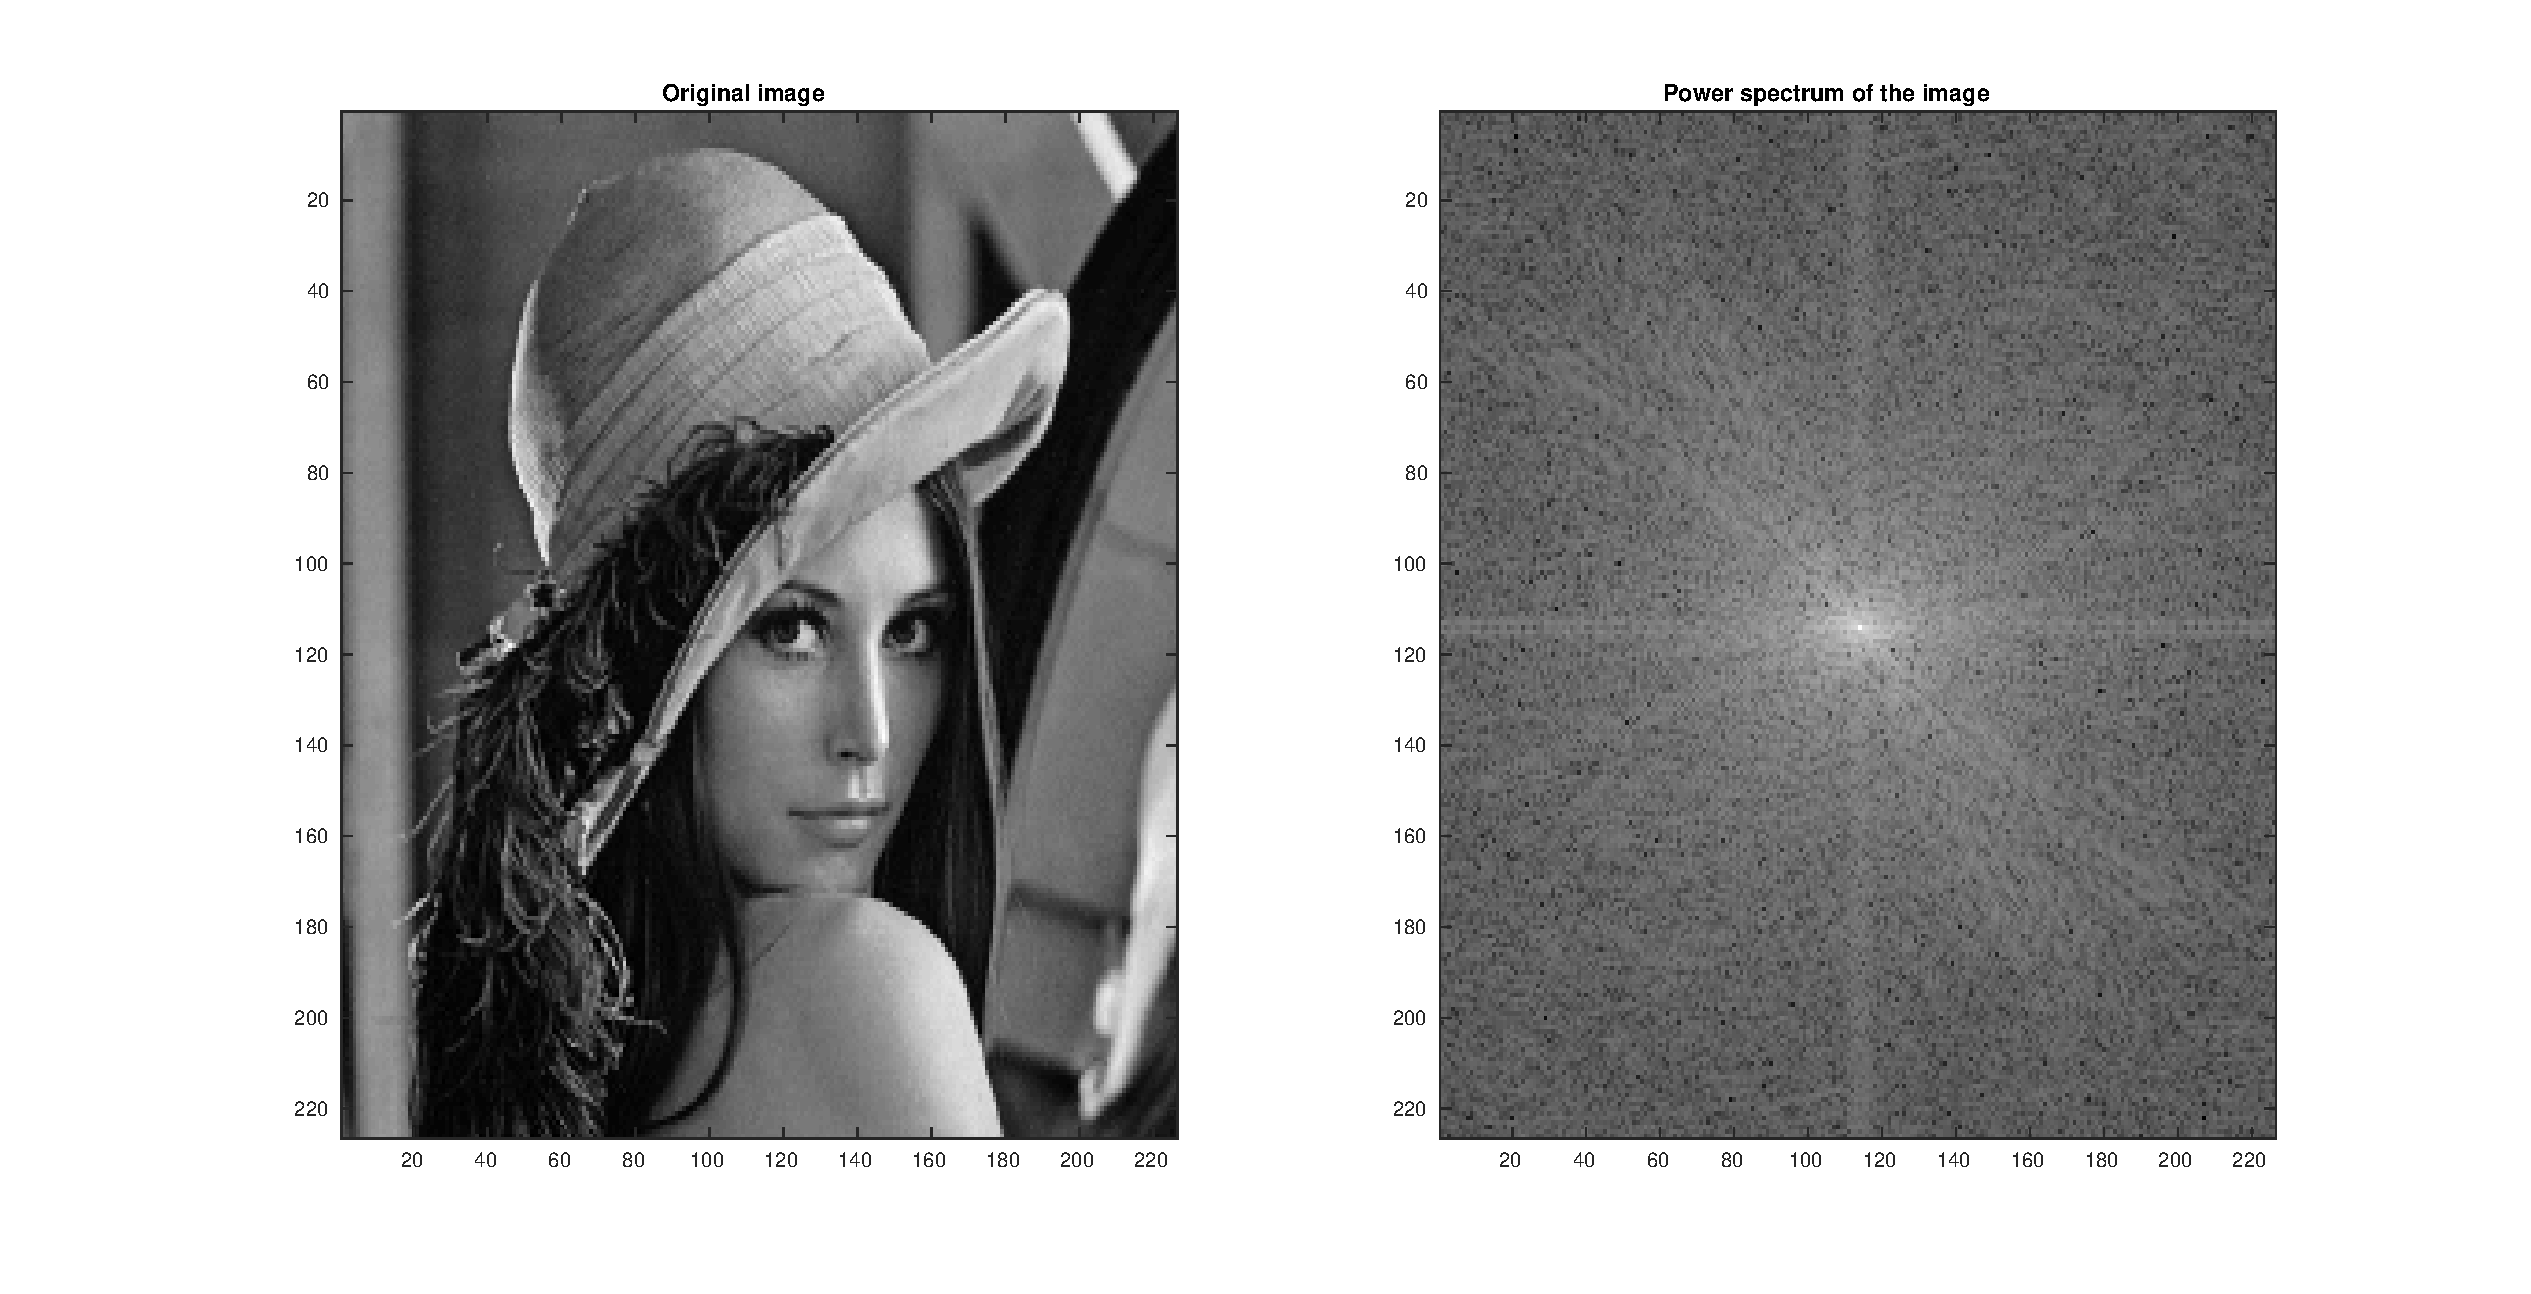
\includegraphics[width=\textwidth]{fig1}
  \caption{Sketch of the level curves of the objection function and the constraints for
  $a=1/3$, $a=1/2$ and $a=1$.}
  \label{fig1}
\end{figure}
As $a$ passes from $1/2$ to $1$, the KKT point $(0,0,1)$ is not a global minimum anymore.

\section*{Question 3}
\subsection*{(a)}
If we write the general KKT conditions for the minimization problem, we get:
\begin{align*}
  x &\leq 0 \comment{Primal feasibility} \\
  0 &= \Delta f(x) + \mu \Delta(x) \comment{Stationarity} \\
  \mu &\geq 0 \comment{Dual feasibility} \\
  \mu x &= 0 \comment{Complementary slackness}
\end{align*}
When $x=0$, all of them are satisfied except:
\begin{align*}
  \mu \geq 0
\end{align*}
which is the only remaining KKT condition.

\section*{Question 4}
\subsection*{(a)}
We have that the quadratic penalty function is:
\begin{align*}
  \Phi(x,\mu) &= f(x) + \sum_{i=1}^q\mu_i\left( c_i(x)\right)^2
\end{align*}
We only have one constraint, so $q=1$, meaning we can omit the summation. Inserting the $f$ and $c$
yields:
\begin{align*}
  \Phi(x,\mu) &= x_1^2+3x_1+x_2^2 +\mu \left(1-x_1\right)^2
\end{align*}
where $\mu>0$ is the penalty parameter.

\subsection*{(b)}
We can rewrite the penalty function to:
\begin{align*}
  \Phi(x,\mu) &=
  \left(1+\mu\right)x_1^2+\left(3-2\mu\right)x_1+x_2^2+\mu
\end{align*}
We can express this as:
\begin{align*}
  \Phi(x,\mu) &= \frac{1}{2}x^TQx-x^Tb+c
\end{align*}
where
\begin{align*}
  Q &= \begin{bmatrix}
          2+2\mu & 0 \\
          0 & 2
       \end{bmatrix} \\
       b &= \begin{bmatrix}
       3-2\mu \\
       0
     \end{bmatrix} \\
     c &= \mu
\end{align*}
The minimizer $x^*(\mu)$ is then given by $Q^{-1}b$:
\begin{align*}
  x^*(\mu) &= Q^{-1}b \\
           &=\begin{bmatrix} -(2\mu-3)/(2\mu+2) \\ 0 \end{bmatrix} \\
           &=\begin{bmatrix} (3-2\mu)/(2\mu+1) \\ 0 \end{bmatrix}
\end{align*}
for $\mu>0$.

\subsection*{(c)}
The partial derivatives are:
\begin{align*}
  \frac{\partial \Phi}{\partial x_1} &= 2x_1+2\mu x_1+3-2\mu \\
  \frac{\partial \Phi}{\partial x_2} &= 2x_2
\end{align*}
So the gradient in a general point $x$ is:
\begin{align*}
\Delta f(x)=\begin{bmatrix} 2x_1+\frac{x_1-1}{\mu}+3 \\ 2x_2 \end{bmatrix}
\end{align*}
Solving for $x$ equal to zero gives us the estimate for $\gamma^*(\mu)$:
\begin{align*}
\gamma^*(\mu)&=\begin{bmatrix} \frac{1-3\mu}{2\mu+1} \\ 0 \end{bmatrix}
\end{align*}
Remember we have $\mu>0$.

\subsection*{(d)}
First we construct the Hessian. The second partial derivatives are:
\begin{align*}
  \frac{\partial^2 \Phi}{\partial x_1^2} &= \frac{1}{a}+2 \\
  \frac{\partial^2 \Phi}{\partial x_1\partial x_2} &= 0 \\
  \frac{\partial^2 \Phi}{\partial x_2\partial x_1} &= 0 \\
  \frac{\partial^2 \Phi}{\partial x_2^2} &= 2
\end{align*}
So the Hessian, $H$, is:
\begin{align*}
  H &= \begin{bmatrix}
         \frac{1}{\mu}+2 & 0 \\
         0 & 2
        \end{bmatrix}
\end{align*}
I am not entirely sure how we can take it in the point $x=x^*(\mu)$ as the Hessian is
constant for quadratic functions.

\subsection*{(e)}
We have the following limits for $\mu\rightarrow \infty$:
\begin{align*}
\lim_{\mu\rightarrow \infty}x^*(\mu)&= \begin{bmatrix} -1 \\ 0 \end{bmatrix} \\
\lim_{\mu\rightarrow \infty}\gamma^*(\mu)&= \begin{bmatrix} -3/2 \\ 0 \end{bmatrix} \\
\lim_{\mu\rightarrow \infty}H&= \begin{bmatrix} 2 & 0 \\ 0 & 2 \end{bmatrix}
\end{align*}
The minimizer and the estimate for the Lagrange multiplier are somewhat similar. That is,
we can expect a rate of change of around $-1$ to $-3/2$ in the objective function as we
relax the constraint $c$. I think my calculations for the Hessian, so I will not comment
too much on that.

\end{document}

